%%%%%%%%%%%%%%%%%%%%%%%%%%  phdsymp_sample2e.tex %%%%%%%%%%%%%%%%%%%%%%%%%%%%%%
%% changes for phdsymp.cls marked with !PN
%% except all occ. of phdsymp.sty changed phdsymp.cls
%%%%%%%%%%                                                       %%%%%%%%%%%%%
%%%%%%%%%%    More information: see the header of phdsymp.cls   %%%%%%%%%%%%%
%%%%%%%%%%                                                       %%%%%%%%%%%%%
%%%%%%%%%%%%%%%%%%%%%%%%%%%%%%%%%%%%%%%%%%%%%%%%%%%%%%%%%%%%%%%%%%%%%%%%%%%%%%%


%\documentclass[10pt]{phdsymp} %!PN
\documentclass[twocolumn]{phdsymp} %!PN
%\documentclass[12pt,draft]{phdsymp} %!PN
%\documentstyle[twocolumn]{phdsymp}
%\documentstyle[12pt,twoside,draft]{phdsymp}
%\documentstyle[9pt,twocolumn,technote,twoside]{phdsymp}

\usepackage[english]{babel}       % Voor nederlandstalige hyphenatie (woordsplitsing)

\usepackage{graphicx}                   % Om figuren te kunnen verwerken
\usepackage{graphics}			% Om figuren te verwerken.
\graphicspath{{figuren/}}               % De plaats waar latex zijn figuren gaat halen.

\usepackage{cleveref}
\usepackage{times}

\hyphenation{si-mu-la-ted re-a-lis-tic packets really in-clu-ding}

\def\BibTeX{{\rm B\kern-.05em{\sc i\kern-.025em b}\kern-.08em
    T\kern-.1667em\lower.7ex\hbox{E}\kern-.125emX}}

\newtheorem{theorem}{Theorem}

\begin{document}

\title{Optimization of client-side intermodal \\route planning} %!PN

\author{Brecht Van de Vyvere}

\supervisor{prof. Erik Mannens, prof. Rik Van de Walle, Pieter Colpaert, dr. ir. Ruben Verborgh}

\maketitle

\begin{abstract}
Linked Connections is a framework that enables clients to calculate public transit routes. A server is responsible for publishing the data as Linked Data Fragments. This article introduces a speedup method that accelerates local queries almost twice as fast while saving a third in bandwidth.
\end{abstract}

\begin{keywords}
Linked Connections, optimization, route planning, client-side, GTFS
\end{keywords}

\section{Introduction}
\PARstart{R}{oute} planning is a well known problem within research groups. There are many types of queries that need to be solved in public transit route planning. This research tries to solve \textit{Earliest Arrival Time} queries. Route planning has been traditionally solved with Dijkstra algorithm \cite{raptor}. This means that public transit networks are modelled as a graph-based network. Dijkstra calculates the shortest path between a source node and every other node. Several optimization techniques have been introduced to achieve query times within microseconds \cite{scalable-transfer-patterns}. Since 2013, the Connection Scan Algorithm (CSA) \cite{csa} makes route planning a data problem, instead of a mathematical one. Until recent \cite{colpaert_iswc_2015}, these algorithms have only been solved on server-side. This means that a route planning API provides clients a ``black box''. Linked Connections is a framework that enables clients to perform the algorithm. This way, servers are only responsible for publishing the data, but clients need to do more heavy lifting. In this paper we discuss a new trade-off on top of the existing Linked Connections implementation to retrieve faster query results.

\section{Linked Connections: concept}

A connection $c$ represents a vehicle that departs in a certain departure stop $c_{depstop}$ and arrives in a certain arrival stop $c_{arrstop}$ without stopping. Also an indication of the departure time $c_{deptime}$ and arrival time $c_{arrtime}$ is contained within a connection. An \textit{Earliest Arrival Time} $query$ exists out of three components: the stop where the route starts $query_{depstop}$, the destination $query_{arrstop}$ and a time of departure $query_{deptime}$. CSA \cite{csa} can calculate such queries by scanning a list of connections sorted by their departure time $c_{deptime}$.
Connections are retrieved out of a \textit{General Transit Feed Specification} (GTFS) feed. This format is widely used by public transit companies to publish their static time schedules.
LC makes use of Linked Data Fragments (\cite{verborgh_ldow_2014}) to publish these connections on the Web. This conceptual framework shows the amount of effort that needs to be done by data consumers and data publishers. A \textit{Linked Connections Fragment} (LCF) contains connections from a subset of stops $S$ from a dataset and hypermedia controls, e.g. to find a next fragment. You can see in \cref{LDF-asFinalAbstract} that LC introduces new trade-offs between client and server by moving intelligence to the client. (1) represents the original implementation of LC. (2) and (3) are respectively the heuristic and speedup optimizations that will be futher discussed in \cref{optimization}. In next subsection, we explain how LC currently publishes its connections with \textit{basic LCFs} (BLCFs).

\begin{figure}[ht]
\begin{center}
	\includegraphics[width=.40\textwidth]{LDF-asFinalAbstract}
	\caption{\label{LDF-asFinalAbstract}Linked Data Fragments-axis for public transit route planning. On the left, you can see data dumps, e.g. GTFS files. On the right, you have web services that provide certain functionality to clients. Linked Connections tries to find new ways to plan routes by publishing transit data using different types of fragments.}
\end{center}
\end{figure}

\subsection{Basic Linked Connections Fragment}

A \textit{basic} LCF (BLCF) contains every connection $c$ that has a departure time between the fragments time interval $F_{start}$ and $F_{end}$. This time interval can be fixed to every $X$ minutes or precalculated so every fragment has a similar size of connections. The subset of stops $S$ of a BLCF contains every stop of the dataset. \Cref{hypermediafragmenten} shows how BLCFs have a \textit{nextPage}-link as hypermedia control to the next fragment.
This way of publishing makes a server scalable, but clients need to scan a lot of connections that are useless, because of $S$. E.g.: when you depart in Brussels, you're not interested in connections from Madrid at that moment. To address this issue, we introduce a new type of LDF in \cref{nlcf}.

\begin{figure}[ht]
\begin{center}
	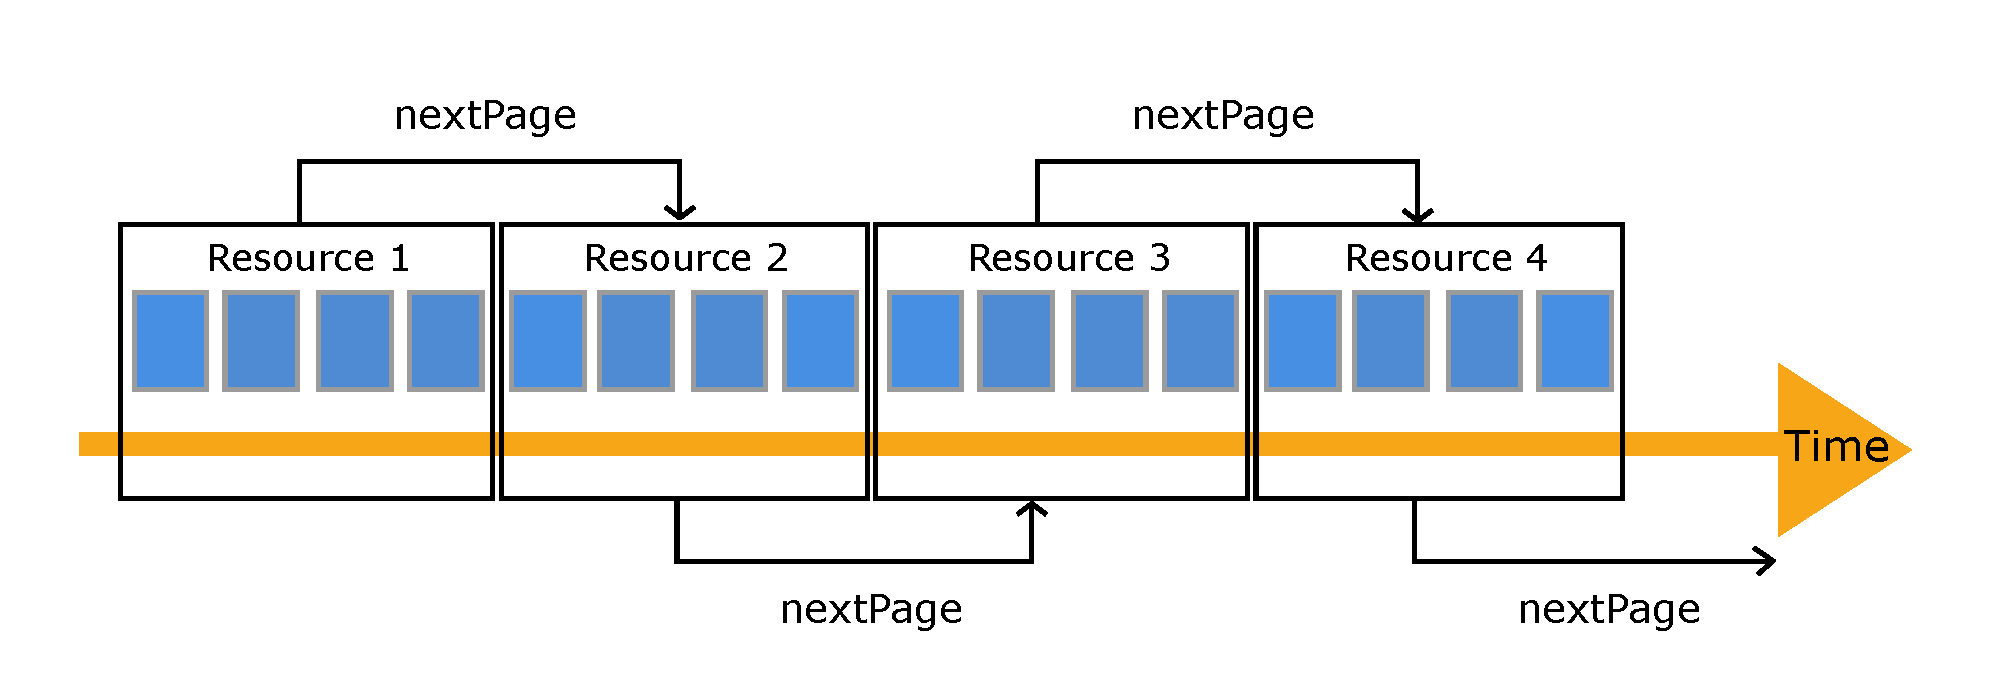
\includegraphics[width=.40\textwidth]{hypermediafragmenten}
	\caption{\label{hypermediafragmenten}A \textit{basic} LCF represents all connections between a certain time range.}
\end{center}
\end{figure}

\subsection{Neighbour Linked Connections Fragment}
\label{nlcf}

In a \textit{neighbour} LCF, connections are returned depending relative to the $query_{deptime}$ and $query_{depstop}$. $S$ represents the $query_{depstop}$ and its neighbours within a certain maximum amount of possible transfers $K_{max}$. Every stop $s$ of $S$ has its own time interval of connections that belong to the fragment.
By providing information about the departure stop, connections can be filtered out by taking the minimum time to reach a neighbouring stop into account. This way, more usefull connections can be returned. A \textit{usefull} connection is a connection that CSA adds to the Minimum Spanning Tree (MST).
Two features need to be pre-processed for every pair stops ($A$, $B$):

\begin{itemize}
\label{prefeatures}
\item The minimum amount of transfers $K(A, B)$ that is needed to reach B from A.
\item The minimum amount of time $R(A, B)$ to get from A to B.
\end{itemize}

\subsubsection{Pre-processing}

Pre-processing of above features (\cref{prefeatures}) requires two additional steps.
\begin{enumerate}
\item Calculate $R(A,B)$ for every pair direct reachable stops $A$ and $B$. A stop is direct reachable if it can be reached within one trip, so $K(A,B) = 0$. This information can be fetched by looping through the \textit{stop\_times.txt} file of a \textit{GTFS} feed or while generating connections.
\item Calculate $R(A,B)$ and $K(A,B)$ for every stop $A$ in the dataset to every indirect ($K(A,B)>0$) reachable stop $B$.
\end{enumerate}

\Cref{table:calcneighbours} shows that the amount of pre-processing time is acceptable.
\begin{table}[htbp]
\centering
\begin{tabular}{ | c || c | c | }
  \hline
  Dataset & Amount of stops & Pre-processing time (min) \\ \hline
  NMBS\footnote{Belgian railway company} & 597 & 6,35 \\
  NS\footnote{Dutch railway company} & 2532 & 21,19 \\
\hline  
\end{tabular}
\caption{Time to calculate indirect reachable stops for every stop in a \textit{GTFS} feed.}
\label{table:calcneighbours}
\end{table}

\section{Optimization}
\label{optimization}

There are two optimizations tested. The first one (\cref{heuristic}) tries to find the fastest route by only using NLCFs. The fastest route is not guaranteed, because a heuristic determines the next fragment. The second optimization (\cref{speedup}) uses the benefits of the heuristic method to speedup the original BLCFs method while guaranteeing the fastest route.

\subsection{Heuristic}
\label{heuristic}

The heuristic method ((2) on \cref{LDF-asFinalAbstract}) tries to solve the fastest route problem by only using NLCFs. Every stop $s$ of the NLCF uses the same time range $T$ (\cref{neighbourconnections}). $T$ and $K_{max}$ can be changed dynamically on the server. The fastest route is found if every connection $c$ of the fastest route has following properties:
\begin{itemize}
\item $query_{deptime} + R(query_depstop, c_{depstop}) <= c_{deptime} < c_{depstop} + T$: $c$ departs within the time range of the stop $c_{depstop}$
\item $c_{depstop} \in S$ with $S$ determined by the maximum amount of transfers $K_{max}$
\end{itemize}

\begin{figure}[ht]
\begin{center}
	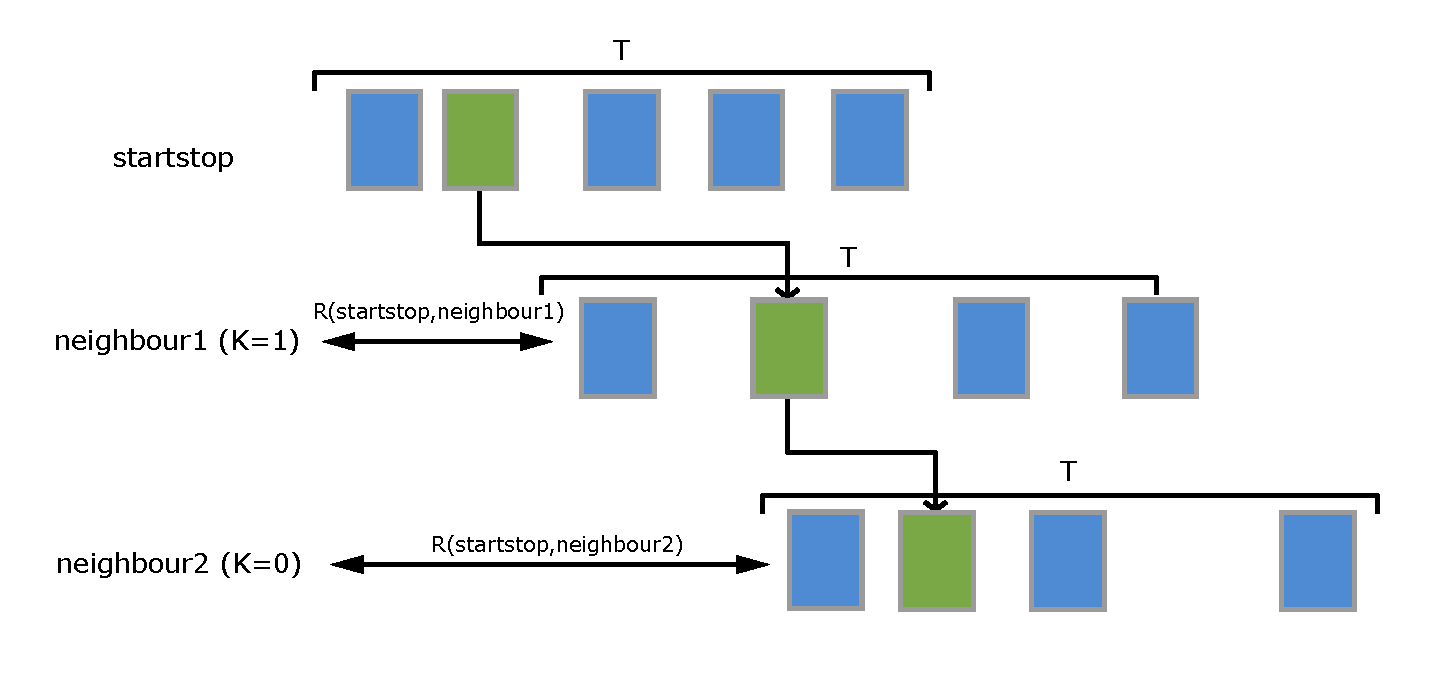
\includegraphics[width=.40\textwidth]{Burenconnecties}
	\caption{\label{neighbourconnections}Overview of connections that are returned within a Neighbour LC Fragment for the heuristic optimization. Note that the amount of stops is limited by a maximum amount of possible transfers $K_{max}$.}
\end{center}
\end{figure}

If the fastest route is not found a next NLCF needs to be fetched by the client. The heuristic method does this by holding a priority queue of reached stops. Every \textit{usefull} connection $c$ is analysed and gets a priority by \cref{priorityfunction}:
\begin{equation} \label{priorityfunction}
priority(c) = \alpha * c_{v} + \beta * c_{arrstop}[importance] + \gamma * \cos(\theta)
\end{equation}

Parameters that are used:
\begin{itemize}
\item \textit{Velocity} $c_{v}$ is distance over time of the connection.
\item \textit{Importance} of a stop is indicated by the amount of direct reachable stops.
\item \textit{Cosine simularity} shows if $c$ is going in the right direction. $\theta$ is the degree between the connection $c$ vector and the vector between $query_{depstop}$ and $query_{arrstop}$.
\end{itemize}

The heuristic method results in a suboptimal solution if a next stop is chosen that doesn't belong to the fastest route and the destination gets reached. It depends of the chosen stop how many minutes longer the route takes. The results (\cref{results}) will show that most queries can be solved with the first NLCF.
Following optimization method combines the use of this first NLCF together with ordinary BLCFs to guarantee the fastest route.

\subsection{Speedup}
\label{speedup}

The speedup method accelerates the original LC implementation by using initial one NLCF. This NLCF is splitted in multiple pages with hypermedia links holding them together (\cref{NLCFpaged}). This way a client only needs to fetch necessary connections and saves bandwidth. The NLCF uses one global time interval $T$ for all the stops.
\begin{figure}[ht]
\begin{center}
	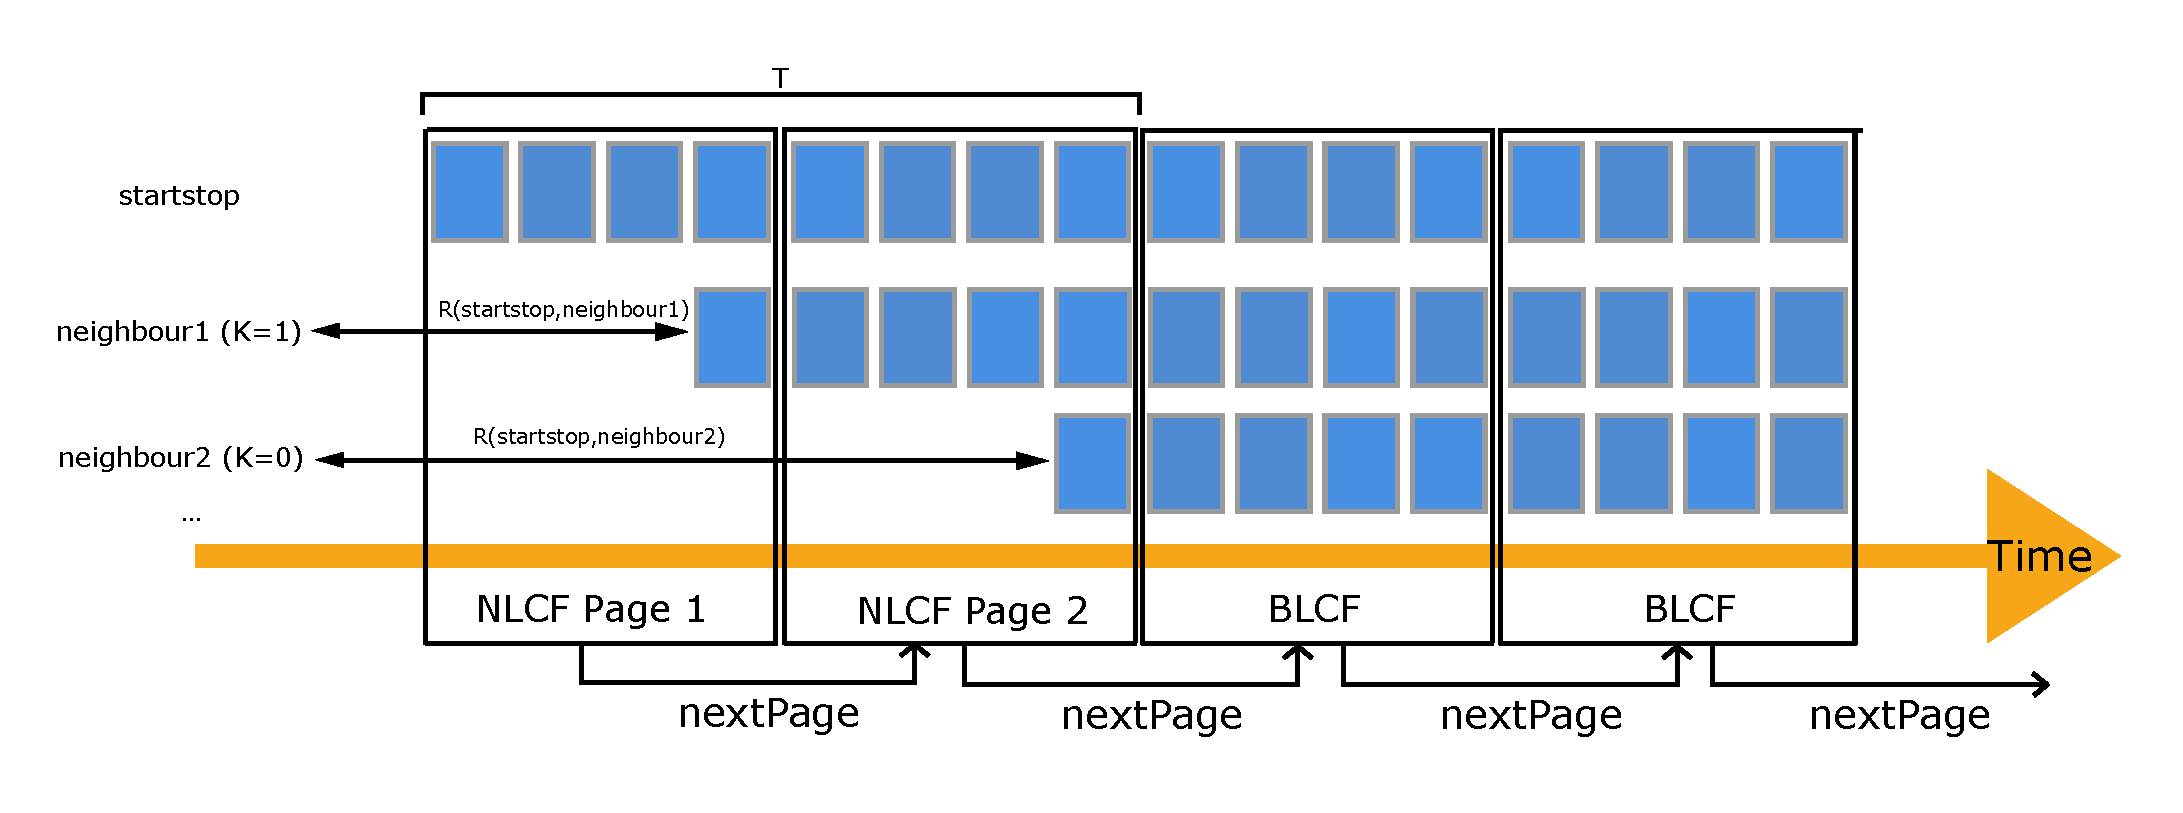
\includegraphics[width=.40\textwidth]{NLCFpaged}
	\caption{\label{NLCFpaged}Overview of the speedup technique. First a NLCF is used to filter connections by the departure time and departure stop of the query. After a certain time period $T$, basic LCFs are used.}
\end{center}
\end{figure}

To guarantee that the fastest route can be found, all stops of the dataset need to be included ($K_{max}$ represents every stop) in the NLCF. After $T$, hypermedia \textit{nextPage}-links refer to ordinary BLCFs. The size of $T$ depends off the dataset. For the NMBS, the Belgian railway company, most stops can be reached within 120 - 150 minutes. There's no big difference with BLCFs after that time.
This speedup method is the most centered line (3) on the LDF-axis (\cref{LDF-asFinalAbstract}) because it requires three HTTP parameters: the departure time, departure stop and page number. This causes less caching possibilities for the server thus higher server effort.

\section{Results}
\label{results}

For testing previous methods (BLCFs, heuristic and speedup) 900 queries are generated. The NMBS GTFS feed is used which contains 644 stops and 127116 connections for one day. All tests have been run on a Macbook Pro 2015 with 8 GB RAM and Intel Core i5 2,7 Ghz CPU. There are still software issues for e.g. stations that are hard to reach, which causes the client to stop searching. The results are representative for local, in Belgium located, stations. 
The time interval of a basic LCF is limited to every 20 minutes, representing 1100 connections on average. Neighbour LCFs of the heuristic method has a time interval of 100 minutes. The NLCF of the speedup method uses a NLCF of 120 minutes splitted in pages of 30 minutes.

\subsection{Speed}

\Cref{timedistancewithcaching} shows the time to plan a route according to the distance of the route in bird flight. The original method (in blue) and speedup method (in red) both grow linear with the distance. It is clear that the speedup method accelerates the original method with seconds. The heuristic method in yellow follows a different pattern. Almost all query times are located on a horizontal line of 2 seconds. This means that these queries are all solved with the first NLCF. Only a few queries are solved with multiple NLCFs. Note that 22\% of the results of the heuristic method are not displayed due to a suboptimal solution.
\begin{figure}[ht]
\begin{center}
	
\includegraphics[width=.40\textwidth]{timedistancewithcaching}
	\caption{\label{timedistancewithcaching}Time to calculate queries according to the distance of the route.}
\end{center}
\end{figure}

\subsection{Bandwidth}

An important aspect of the optimization is bandwidth. The speedup method clears useless connections in the beginning. You can see in \cref{datausagedistance} how data consumption has been lowered. The use of hypermedia makes sure that the amount of downloaded connections can be minimized with 38\%.
\begin{figure}[ht]
\begin{center}
	
\includegraphics[width=.40\textwidth]{datausagedistance}
	\caption{\label{datausagedistance}Overview of bandwidth consumption. An extra filter by departure stop ensures more usefull connections per request, so less bandwidth.}
\end{center}
\end{figure}

\Cref{table:summary} gives a summary of the results regarding speed, data consumption and usefull connnections.
\begin{table}[htbp]
\centering
\begin{tabular}{ | l || c | c | c |}
\hline
  & Basic & Speedup & Heuristic  \\ \hline
  Speed with caching (s) & 4.54 & 2.87 & 1.96 \\
  Data usage (MB) & 2.69 & 1.68 & 1.97 \\
  Usefull connections (\%) & 0.026 & 0.047 & 0.064 \\
  Optimal & yes & yes & no \\
\hline  
\end{tabular}
\caption{}
\label{table:summary}
\end{table}

\section{Conclusion}
We have tested how fast the current implementation with only \textit{basic} Linked Connections Fragments works. To make this faster, we introduced two different methods that use an extra filter based on the departure stop and departure time of the query. Pre-processing time is limited to minutes. The heuristic method works the fastest, but only returns the optimal result for 78\% of the tested queries. The speedup method makes route planning almost twice as fast while guaranteeing the optimal solution. Also bandwidth is saved by 38\%. We can conclude that this research succeeds in optimizing client-side route planning with Linked Connections.

\nocite{*}
\bibliographystyle{phdsymp}
%%%%%\bibliography{bib-file}  % commented if *.bbl file included, as
%%%%%see below


%%%%%%%%%%%%%%%%% BIBLIOGRAPHY IN THE LaTeX file !!!!! %%%%%%%%%%%%%%%%%%%%%%%%
%% This is nothing else than the phdsymp_sample2e.bbl file that you would%%
%% obtain with BibTeX: you do not need to send around the *.bbl file        
%%
%%---------------------------------------------------------------------------%%
%
\begin{thebibliography}{1}

\bibitem{raptor}
Daniel Delling and Thomas Pajor and Renato F. Werneck,
\newblock {\em Round-Based Public Transit Routing },
\newblock { Transportation Science, pages 591-604, 2015}

\bibitem{scalable-transfer-patterns}
Hannah Bast and Matthias Hertel and Sabine Storandt,
\newblock {\em Scalable Transfer Patterns},
\newblock { 2016 Proceedings of the Eighteenth Workshop on Algorithm Engineering and Experiments (ALENEX) }

\bibitem{csa}
Dibbelt, Julian and Pajor, Thomas and Strasser, Ben and Wagner, Dorothea,
\newblock {\em Intriguingly Simple and Fast Transit Routing},
\newblock {Experimental Algorithms, pages 43-54,. Springer, 2013. }

\bibitem{colpaert_iswc_2015}
Colpaert, Pieter and Llaves, Alejandro and Verborgh, Ruben and Corcho, Oscar and Mannens, Erik and Van de Walle, Rik,
\newblock {\em Intermodal public transit routing using {Linked Connections}},
\newblock {Proceedings of the 14th International Semantic Web Conference: Posters and Demos, oct. 2015}

\bibitem{verborgh_ldow_2014}
Verborgh, Ruben and Vander Sande, Miel and Colpaert, Pieter and Coppens, Sam and Mannens, Erik and Van de Walle, Rik,
\newblock {\em Web-Scale Querying through {Linked Data Fragments} },
\newblock {Proceedings of the 7th Workshop on Linked Data on the Web, apr. 2014}


\bibitem{gtfs-ref}
\newblock {\em GTFS reference},
\newblock https://developers.google.com/transit/gtfs/reference

\end{thebibliography}
%
%%---------------------------------------------------------------------------%%

\end{document}

%%%%%%%%%%%%%%%%%%%%%  End of phdsymp_sample2e.tex  %%%%%%%%%%%%%%%%%%%%%%%%%%%
